\documentclass{standalone}
\usepackage{tikz}
\usetikzlibrary{fit,shapes}
\begin{document}
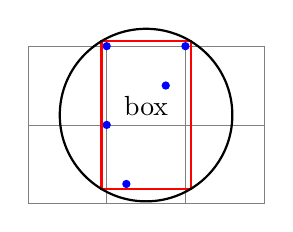
\begin{tikzpicture}[inner sep=0pt,thick,
dot/.style={fill=blue,circle,minimum size=3pt}]
\draw[help lines] (0,0) grid (3,2);
\node[dot] (a) at (1,1) {};
\node[dot] (b) at (2,2) {};
\node[dot] (c) at (1,2) {};
\node[dot] (d) at (1.25,0.25) {};
\node[dot] (e) at (1.75,1.5) {};
\node[draw=red, fit=(a) (b) (c) (d) (e)] {box};
\node[draw,circle,fit=(a) (b) (c) (d) (e)] {};
\end{tikzpicture}

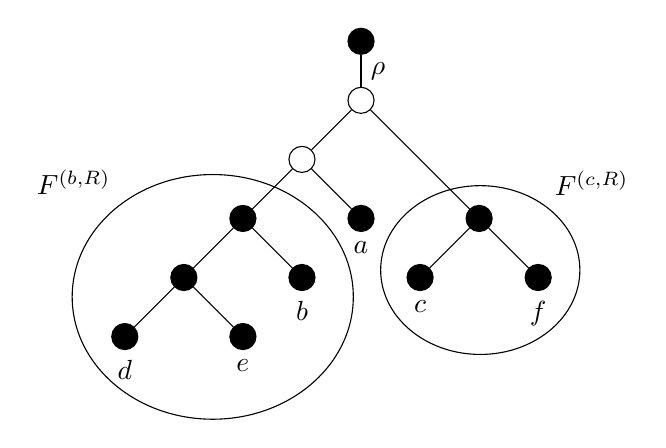
\begin{tikzpicture}
[vertex/.style={minimum size=2pt,fill,draw,circle},
open/.style={fill=none},
sibling distance=1.5cm,level distance=.75cm,
every fit/.style={ellipse,draw,inner sep=-2pt},
leaf/.style={label={[name=#1]below:$#1$}},auto]
\node [vertex] (root) {}
child { node [vertex,open] {}
child { node [vertex,open] {}
child { node [vertex] (b's parent) {}
child { node [vertex] {}
child { node [vertex,leaf=d] {} }
child { node [vertex,leaf=e] {} } }
child { node [vertex,leaf=b] {} } }
child { node [vertex,leaf=a] {} } }
child { node [coordinate] {}
child[missing]
child { node [vertex] (f's parent) {}
child { node [vertex,leaf=c] {} }
child { node [vertex,leaf=f] {} } } }
edge from parent node {$\rho$} };
\node [fit=(d) (e) (b) (b's parent),label=above left:$F^{(b,R)}$] {};
\node [fit=(c) (f) (f's parent),label=above right:$F^{(c,R)}$] {};
\end{tikzpicture}
\end{document}